\clearpage
\subsection{Type} % (fold)
\label{sub:type}

All values within a program will have a Type. The Type indicates how the data stored in the computers memory is interpreted by the program. There are three basic data Types available in a programming language.

\begin{itemize}
    \item \textbf{Textual} data such as `\emph{Fred}', `\emph{Hello World}', `\emph{23}', and `\emph{This is text!}'.
    \item \textbf{Whole numbers} such as \emph{1}, \emph{0}, \emph{-5}, and \emph{37}.
    \item \textbf{Real numbers} such as \emph{0.5}, \emph{-126.0}, \emph{3.141516}, and \emph{23.981}.
\end{itemize}

\begin{figure}[h]
   \centering
   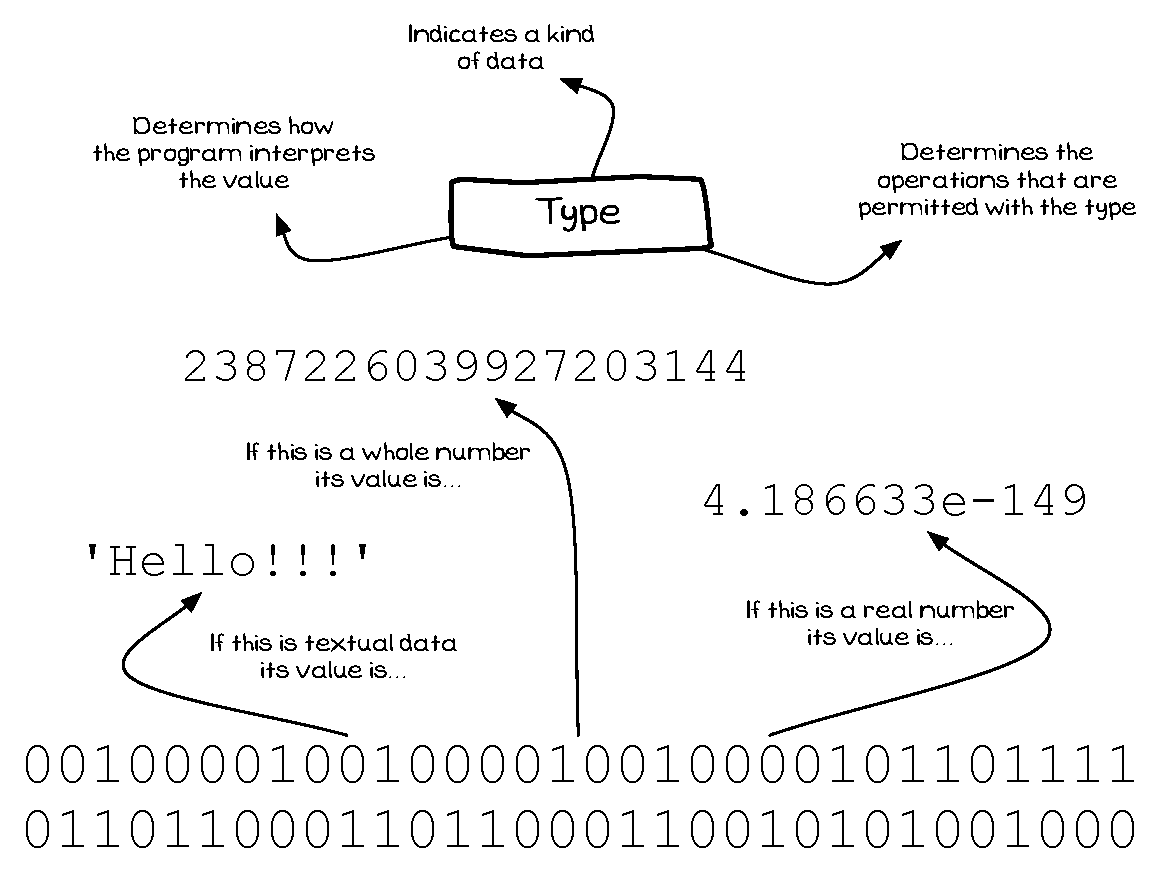
\includegraphics[width=\textwidth]{./topics/program-creation/diagrams/Type} 
   \caption[Type Concept Diagram]{Types defines how values are interpreted, and the operations that can be performed on the data}
   \label{fig:program-creation-type}
\end{figure}

\mynote{
\begin{itemize}
  \item The concepts related to Expressions are shown in Figure \ref{fig:program-creation-type}.
  \item A Type is a programming artefact that indicates a kind of data.
  \item The type determines the basic actions that can be performed on the value.
  \item The type determines the amount of memory needed to store a value of that kind.
  \item Whole numbers are usually called \textbf{Integers}.
  \item Real numbers are usually represented as \textbf{Floating Point} values. These values have a limited precision, supporting only a certain number of digits of precision.
  \item Textual values can contain numbers. In these cases the number are just textual representations of the values. For example, the text `\emph{23}' is the character `\emph{2}' followed by the character `\emph{3}', it is not the number \emph{23}.
  \item You can perform mathematic operations on numeric data, but not on textual data.
\end{itemize}
}

% section program (end)